\documentclass[
fontsize=12pt,          % Schriftgröße
paper=a4,               % Papiergröße
captions=tableabove,    % Beschriftungen für Tabellen oberhalb
titlepage=firstiscover, % Titelseite ist Umschlagseite
BCOR=5mm,               % Korrektur für Bundsteg
toc=listof,             % Abbildungs- und Tabellenverzeichnis im Inhaltsverzeichnis
open=right,             % Kapitel beginnen auf rechter Seite
]{scrreprt}

% requires: \usepackage{tikz}
% requires: \usetikzlibrary{arrows}
\usepackage{tikz}
\usetikzlibrary{arrows}
\usepackage{german}
\usepackage[utf8]{inputenc}

% diagram packages
\usepackage{siunitx}
\usepackage{pgfplots}

\pgfplotsset{compat=newest} % Allows to place the legend below plot
\usepgfplotslibrary{units} % Allows to enter the units nicely

\begin{document}
	
\chapter{Aufgabe 1}

\section{Beschriftung der Abbildung}

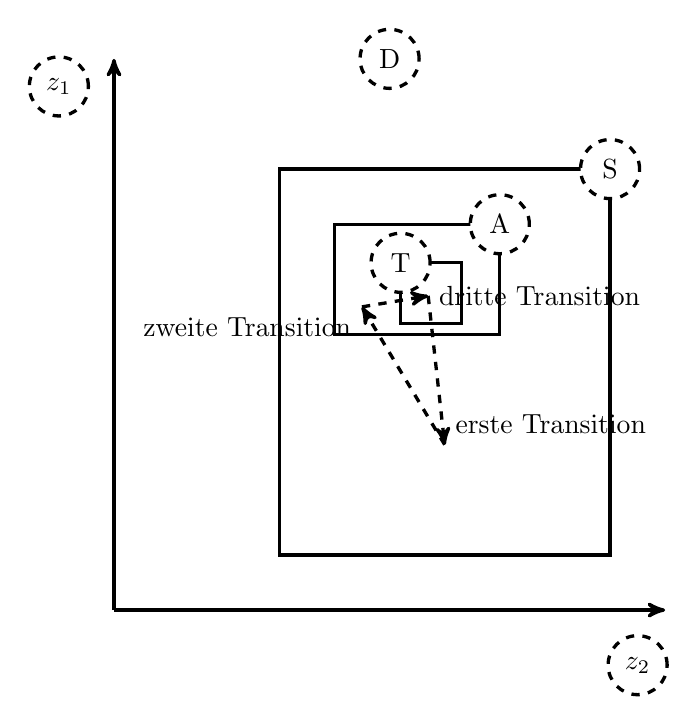
\begin{tikzpicture}[
  >=stealth',
  very thick,
  scale=0.7,
  gap/.style={draw,circle,minimum width=0.75cm,inner sep=0,dashed,fill=white,align=center}
  ]


  \draw[->] (0, 0) -- (0, 10);
  \node [gap] at (-1, 9.5) {$z_1$};
  \draw[->] (0, 0) -- (10, 0);
  \node [gap] at (9.5, -1) {$z_2$};


  \node [gap] at (5, 10) {D};
  \draw (3, 1) rectangle (9, 8) node [gap] {S};
  \draw (4, 5) rectangle (7, 7) node [gap] {A};
  \draw (5.2, 5.2) rectangle (6.3, 6.3);
  \node [gap] at (5.2, 6.3) {T};
  \draw[->,dashed] (5.7, 5.7) -- (6, 3) node[anchor=south west]{erste Transition};
  \draw[->,dashed] (6, 3) -- (4.5, 5.5) node[anchor=north east]{zweite Transition};
  \draw[->,dashed] (4.5, 5.5) -- (5.7, 5.7) node[anchor=west] {dritte Transition};
  
\end{tikzpicture}

\section{Zuordnung der Situationen}
\begin{enumerate}
	\item Target Space, global optimaler Zustand, keine technischen Mängel
	\item Transition von Target Space zu Survival Space, Einfluss der Umgebung löst Störung aus, im Survival Space ist die Rückkher in den Acceptance Space aber noch möglich (kein Unfall)
	\item Transition von Survival Space zu Acceptance Space, Kontrollmechanismus löst Korrektur des Systems aus
	\item Acceptance Space, da eingeschränkter Betrieb des Fahrzeug möglich ist
	\item Transition von Acceptance Space zu Target Space, da weitere Korrekturmaßnahmen (Besuch der Werkstatt) durchgeführt werden
	\item Target Space, uneingeschränkte Nutzung des Fahrzeug ist wieder möglich
\end{enumerate}

\section{Terminologie}
\begin{enumerate}
	\item das System befindet sich dann im Survival Space, da die aktuelle Geschwindigkeit 180 kmh beträgt und die Akzeptanzkriterien aber auf eine neue Position bewegt wurden
	\item Ja, das System ist robust bezüglich eines Staus, da in einem Stau die Weiterfahrt möglich ist, allerdings nur mit eingeschränkter Geschwindigkeit (Acceptance Space). die Robustheit ist aktiv, da das Tempo beschleunigt wird, sobald die Störung (der Stau) nicht mehr besteht. Im Zusammenhang mit Aufgabe 1.1 macht es mehr Sinn von Flexibilität zu sprechen. Da das Fahrzeug eine Bremse besitzt, kann es flexibel genannt werden.
	\item Ein Beispiel für Flexibilität ist das Überschreiten der Landesgrenzen, da andere Länder andere Geschwindigkeitsbegrenzungen festlegen und der Acceptance Space sich verschiebt und dann nicht mehr bei 180 kmh liegt.
	\item 1. Transition: Überqueren der Staatsgrenze, Übergang vom Target zum Survival Space. 2. Transition: Bremsen des Fahrzeugs, Übergang von Survival zum Target Space.
	\item Transitionen durch Flexibilität:\newline\newline
	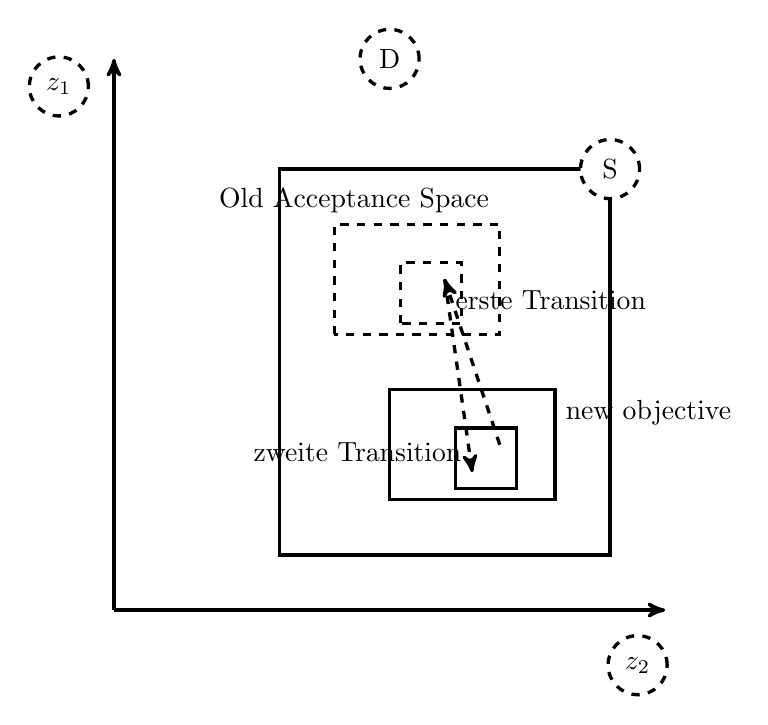
\begin{tikzpicture}[
	>=stealth',
	very thick,
	scale=0.7,
	gap/.style={draw,circle,minimum width=0.75cm,inner sep=0,dashed,fill=white,align=center}
	]	
	\draw[->] (0, 0) -- (0, 10);
	\node [gap] at (-1, 9.5) {$z_1$};
	\draw[->] (0, 0) -- (10, 0);
	\node [gap] at (9.5, -1) {$z_2$};	
	\node [gap] at (5, 10) {D};
	\draw (3, 1) rectangle (9, 8) node [gap] {S};
	\draw[dashed] (4, 5) rectangle (7, 7) node [anchor=south east] {Old Acceptance Space};
	\draw[dashed] (5.2, 5.2) rectangle (6.3, 6.3);
	\draw (5,2) rectangle (8,4) node[anchor=north west]{new objective}; %node [gap] {A};
	\draw (6.2,2.2) rectangle (7.3,3.3);
	%\node [gap] at (5.2, 6.3) {T};
	%\node [gap] at (6.2,3.3) {T};
	\draw[->,dashed] (7, 3) -- (6, 6) node[anchor=north west]{erste Transition};
	\draw[->,dashed] (6, 6) -- (6.5, 2.5) node[anchor=south east]{zweite Transition};
	%\draw[->,dashed] (6, 3) -- (4.5, 5.5) node[anchor=north east]{zweite Transition};
	%\draw[->,dashed] (4.5, 5.5) -- (5.7, 5.7) node[anchor=west] {dritte Transition};	
	\end{tikzpicture}
\end{enumerate}

\chapter{Aufgabe 3}
\begin{figure}[htb]
	%\begin{center}
		\begin{tikzpicture}[scale=0.5]
		\begin{axis}[
		%width=20cm, % Scale the plot to \linewidth		
		grid=major, % Display a grid
		grid style={dashed,gray!30}, % Set the style
		xlabel=Iteration, % Set the labels
		ylabel=Kosten,
		%x unit=\si{\volt}, % Set the respective units
		%y unit=\si{\ampere},
		legend style={at={(0.5,-0.2)},anchor=north}, % Put the legend below the plot
		x tick label style={rotate=90,anchor=east} % Display labels sideways
		]
		\addplot 
		% add a plot from table; you select the columns by using the actual name in
		% the .csv file (on top)
		table[x=iteration,y=value,col sep=comma] {/home/giuliano/Dokumente/SS20/OC2/abgabe/sheet04/bb0.csv}; 
		%\legend{Plot}
		\end{axis}
		\end{tikzpicture}
		\caption{Blackbox 1}
		\begin{tikzpicture}[scale=0.5]
		\begin{axis}[
		%width=\linewidth, % Scale the plot to \linewidth
		grid=major, % Display a grid
		grid style={dashed,gray!30}, % Set the style
		xlabel=Iteration, % Set the labels
		ylabel=Kosten,
		%x unit=\si{\volt}, % Set the respective units
		%y unit=\si{\ampere},
		legend style={at={(0.5,-0.2)},anchor=north}, % Put the legend below the plot
		x tick label style={rotate=90,anchor=east} % Display labels sideways
		]
		\addplot 
		% add a plot from table; you select the columns by using the actual name in
		% the .csv file (on top)
		table[x=iteration,y=value,col sep=comma] {/home/giuliano/oc2-mango/Blatt04/bb1.csv}; 
		%\legend{Plot}
		\end{axis}
		\end{tikzpicture}
		\caption{Blackbox 2}
	%\end{center}
\end{figure}

\begin{figure}[h!]
	\begin{center}
		\begin{tikzpicture}
		\begin{axis}[
		width=\linewidth, % Scale the plot to \linewidth
		grid=major, % Display a grid
		grid style={dashed,gray!30}, % Set the style
		xlabel=Iteration, % Set the labels
		ylabel=Kosten,
		%x unit=\si{\volt}, % Set the respective units
		%y unit=\si{\ampere},
		legend style={at={(0.5,-0.2)},anchor=north}, % Put the legend below the plot
		x tick label style={rotate=90,anchor=east} % Display labels sideways
		]
		\addplot 
		% add a plot from table; you select the columns by using the actual name in
		% the .csv file (on top)
		table[x=iteration,y=value,col sep=comma] {/home/giuliano/oc2-mango/Blatt04/bb1.csv}; 
		%\legend{Plot}
		\end{axis}
		\end{tikzpicture}
		\caption{Blackbox 2}
	\end{center}
\end{figure}

\begin{figure}[h!]
	\begin{center}
		\begin{tikzpicture}
		\begin{axis}[
		width=\linewidth, % Scale the plot to \linewidth
		grid=major, % Display a grid
		grid style={dashed,gray!30}, % Set the style
		xlabel=Iteration, % Set the labels
		ylabel=Kosten,
		%x unit=\si{\volt}, % Set the respective units
		%y unit=\si{\ampere},
		legend style={at={(0.5,-0.2)},anchor=north}, % Put the legend below the plot
		x tick label style={rotate=90,anchor=east} % Display labels sideways
		]
		\addplot 
		% add a plot from table; you select the columns by using the actual name in
		% the .csv file (on top)
		table[x=iteration,y=value,col sep=comma] {/home/giuliano/oc2-mango/Blatt04/bb2.csv}; 
		%\legend{Plot}
		\end{axis}
		\end{tikzpicture}
		\caption{Blackbox 3}
	\end{center}
\end{figure}

\begin{figure}[h!]
	\begin{center}
		\begin{tikzpicture}
		\begin{axis}[
		width=\linewidth, % Scale the plot to \linewidth
		grid=major, % Display a grid
		grid style={dashed,gray!30}, % Set the style
		xlabel=Iteration, % Set the labels
		ylabel=Kosten,
		%x unit=\si{\volt}, % Set the respective units
		%y unit=\si{\ampere},
		legend style={at={(0.5,-0.2)},anchor=north}, % Put the legend below the plot
		x tick label style={rotate=90,anchor=east} % Display labels sideways
		]
		\addplot 
		% add a plot from table; you select the columns by using the actual name in
		% the .csv file (on top)
		table[x=iteration,y=value,col sep=comma] {/home/giuliano/oc2-mango/Blatt04/bb3.csv}; 
		%\legend{Plot}
		\end{axis}
		\end{tikzpicture}
		\caption{Blackbox 4}
	\end{center}
\end{figure}

\begin{figure}[h!]
	\begin{center}
		\begin{tikzpicture}
		\begin{axis}[
		width=\linewidth, % Scale the plot to \linewidth
		grid=major, % Display a grid
		grid style={dashed,gray!30}, % Set the style
		xlabel=Iteration, % Set the labels
		ylabel=Kosten,
		%x unit=\si{\volt}, % Set the respective units
		%y unit=\si{\ampere},
		legend style={at={(0.5,-0.2)},anchor=north}, % Put the legend below the plot
		x tick label style={rotate=90,anchor=east} % Display labels sideways
		]
		\addplot 
		% add a plot from table; you select the columns by using the actual name in
		% the .csv file (on top)
		table[x=iteration,y=value,col sep=comma] {/home/giuliano/oc2-mango/Blatt04/bb4.csv}; 
		%\legend{Plot}
		\end{axis}
		\end{tikzpicture}
		\caption{Blackbox 5}
	\end{center}
\end{figure}

\end{document}